\chapter{BACKGROUND}

We present the shared prerequisites to our articles.


\section{Deep Learning}

Deep learning is a subfield of machine learning that uses neural
networks.

Feedforward neural networks (FNNs) can be expressed as
$\vec{h}_i = f_i({\matr{W}_i}^\intercal \vec{h}_{i - 1} + \vec{b}_i)$, where
$\vec{h}_i$ is a hidden unit, $\matr{W}_i$ is the weight matrix of layer~$i$ of
the neural network, $\vec{b}_i$ is a bias vector and $f_i$ is a non-linearity
or link function, such as the sigmoid function $f(x) = 1/(1 + e^{-x})$.


\section{Convolutional Neural Networks (CNNs)}

Convolutional neural networks (CNNs) are a type of neural network designed to
model data that is arranged in a grid, as the pixels in an image are arranged.
While each neuron in a layer of an FNN is connected to all neurons in its
previous layer via a matrix multiplication, neurons in a layer of a CNN are
only locally connected to neurons in the previous layer.

We explain the meaning of ``locally connected''. We assume that a given layer
has a 3-D tensor $\tens{V}$ as input, where in addition to the single dimension
of the hidden unit vector $\vec{h}$ of FNNs, there are two extra spatial
dimensions (e.g. $x$ and $y$ dimensions of an image).  A CNN connects the input
tensor $\tens{V}$ to an output tensor $\tens{Z}$ through a 4-D tensor
$\tens{K}$ called a ``kernel'', which contains the CNN's learned parameters.

The kernel has one dimension matching the ``channels'' (the third, i.e.\
non-spatial, dimension of the input tensor $\tens{V}$), one dimension that
becomes the channels of the output tensor $\tens{Z}$, and two spatial
dimensions that are normally much smaller than the input feature tensor
$\tens{Z}$'s spatial dimensions. E.g.\ for an input image of dimensions $224
\times 224$ pixels and~\num{3} colour channels, a CNN kernel's spatial
dimensions would normally be $3 \times 3$. The CNN kernel's weights are thus
shared spatially, and each element of the output tensor is contributed to only
by a $3 \times 3$ spatial region of the input tensor, via a sum over
channel-wise matrix multiplications of the kernel strictly over that spatial
region.

Formally, each element $\tens{Z}_{i, j, k}$ of the output tensor corresponds to the
sum given in Equation~\ref{eqn:convolution}, where~$i$ is the index of the
output channel and $j$ and $k$ are the spatial indices of the output element.
The index~$l$ runs over the input channels, while~$m$ and $n$ are restricted by
the spatial dimensions of the kernel, e.g.\ in our $3 \times 3$ kernel example
we have $m, n \in \{-1, 0, 1\}$.

\begin{equation}
        \tens{Z}_{i, j, k} = \sum_{l, m, n} \tens{V}_{l, j + m, k + n} \tens{K}_{i, l, m, n}
\label{eqn:convolution}
\end{equation}

\begin{figure}
\centering
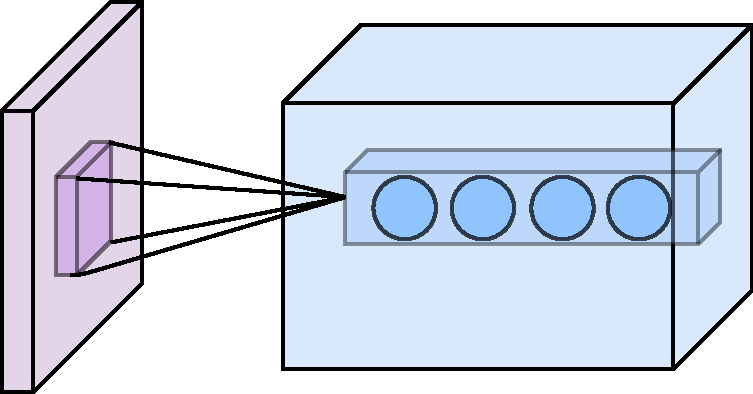
\includegraphics[width=1.0\textwidth]{Figures/cnn.pdf}
\caption{Two subsequent layers of a convolutional neural network.}
\label{fig:cnn}
\end{figure}

Figure~\ref{fig:cnn} depicts the interaction between two subsequent layers of a
CNN\@. The kernel~$\tens{K}$ (inner box on the left) is multiplied with a
volume of the input~$\tens{V}$ (outer box on the left) to produce a single unit
consisting of a column of values at a single spatial location in the
output~$\tens{Z}$.

CNNs generalize well in comparison to FNNs on visual data, since the number of
parameters are dramatically reduced compared with an equivalent FNN by sharing
parameters in the spatial dimensions~\cite{lecun-89}. This is an example of
improving generalization of neural networks by using prior knowledge (i.e.\ in
this case, the spatial invariance of image data) when constructing a model for
a given type of data.

In the case of the visual question-answering task, we make use of a particular
CNN architecture called a ResNet~\cite{he2016deep} that has~\num{152} layers.
This CNN architecture has been pre-trained on a large dataset of image data to
extract useful generic feature representations from images.
The fusion operator takes this image feature representation as input, along
with a feature representation of the question, in order to predict an answer to
the posed question conditioned on the image.


\section{Recurrent Neural Networks (RNNs)}

Like CNNs, Recurrent Neural Networks~(RNNs)~\cite{rumelhart1986learning} are a
type of neural network model that has been invented using prior knowledge of
the type of data distribution relevant to the given task.
In particular, RNNs are designed to work on sequential data of arbitrary
length, such as time-series data including stock prices over time, or language
data, where the inputs are the word or character tokens making up sentences and
paragraphs.

Instead of sharing parameters spatially as in CNNs, RNNs share parameters over
time. The output at each timestep~$t$, $\vect{a}{t}$, takes as input both the
``hidden state'' from the previous timestep~$\vect{h}{t - 1}$ as well as the
input~$\vect{x}{t}$ of the current timestep, as given by
Equation~\ref{eqn:vanilla-rnn}.

\begin{equation}
        \vect{a}{t} = \matr{W}\vect{h}{t - 1} + \matr{U}\vect{x}{t} + \vec{b}
\label{eqn:vanilla-rnn}
\end{equation}

The hidden state~$\vect{h}{t}$ is related to the output~$\vect{a}{t}$ of a
given timestep~$t$ by the link function $f$, i.e.\
$\vect{h}{t} = f(\vect{a}{t})$, where $f$ is usually~$\tanh$.


\section{Skip-Thought Vectors}

Skip-thought vectors~\cite{kiros2015skip} is a method of encoding a feature
representation from a sentence, in such a way that the feature representation
can be re-used as a generic, continuous sentence representation in a variety of
tasks.
In skip-thought vectors, an ``encoder'' RNN is trained to extract a feature
representation with enough context from the current sentence in order to
predict words in the sentences immediately preceding and following the current
sentence.

As their basic neural network component, skip-thought vectors use a type of RNN
called a Gated Recurrent Unit (GRU)~\cite{cho2014ontheproperties}.
The GRU is similar to the vanilla RNN given by Equation~\ref{eqn:vanilla-rnn},
except that there are extra outputs $\vect{r}{t}$ and $\vect{z}{t}$ (and
corresponding weight matrices $\matr{W}_r$, $\matr{U}_r$ and $\matr{W}_z$,
$\matr{U}_z$) that are used to ``turn on or off'' both the contribution of the
hidden state~$\vect{h}{t - 1}$ in Equation~\ref{eqn:vanilla-rnn}, and to
control the update of the hidden state from timestep~$t - 1$ to $t$, as given
by Equation~\ref{eqn:gru-update}.

\begin{equation}
        \vect{h}{t} = (1 - \vect{z}{t}) \odot \vect{h}{t - 1} + \vect{z}{t} \odot \vect{\widetilde{h}}{t}
\label{eqn:gru-update}
\end{equation}

In Equation~\ref{eqn:gru-update},
$\vect{z}{t} = \sigma(\matr{U}_z\vect{h}{t - 1} + \matr{W}_z\vect{x}{t})$,
where $\sigma(\cdot)$ is the sigmoid function. So,
Equation~\ref{eqn:gru-update} is a linear interpolation controlled by the
``update gate'' $\vect{z}{t}$ between the previous hidden state
$\vect{h}{t - 1}$ and the would-be current
hidden-state~$\vect{\widetilde{h}}{t}$.

Regardless of the specific details of GRUs, the relevance to this paper is that
skip-thought vectors use an RNN as an encoder, which encodes the sequence
of words in a sentence into a feature representation corresponding to that
sentence, where the feature representation is a vector of real-valued numbers.

In this work, skip-thought vectors are used to extract a feature representation
from the question, which is coupled with the feature representation extracted
from the image as a dual input to a multi-modal fusion operator, which takes
the two feature-representation inputs and produces an output prediction as to
the answer to the given question, conditioned on the image.


\section{Attention}


\section{Fusion}
